\documentclass[journal]{IEEEtran}

%\usepackage[brazil]{babel}
%\usepackage[T1]{fontenc}

\usepackage{theorem}        %%Lo agregue yo <========================================
\usepackage{algorithmic}        %%Lo agregue yo <========================================

\setcounter{secnumdepth}{7}

\newtheorem{theorem}{Theorem}
\newtheorem{acknowledgement}[theorem]{Acknowledgement}
%\newtheorem{algorithm}[theorem]{Algorithm}
\newtheorem{axiom}[theorem]{Axiom}
\newtheorem{case}[theorem]{Case}
\newtheorem{claim}[theorem]{Claim}
\newtheorem{conclusion}[theorem]{Conclusion}
\newtheorem{condition}[theorem]{Condition}
\newtheorem{conjecture}[theorem]{Conjecture}
\newtheorem{corollary}[theorem]{Corollary}
\newtheorem{criterion}[theorem]{Criterion}
\newtheorem{definition}[theorem]{Definition}
\newtheorem{example}[theorem]{Example}
\newtheorem{exercise}[theorem]{Exercise}
\newtheorem{lemma}[theorem]{Lemma}
\newtheorem{notation}[theorem]{Notation}
\newtheorem{problem}[theorem]{Problem}
\newtheorem{proposition}[theorem]{Proposition}
\newtheorem{remark}[theorem]{Remark}
\newtheorem{solution}[theorem]{Solution}
\newtheorem{summary}[theorem]{Summary}
\newenvironment{proof}[1][Proof]{\textbf{#1.} }{\ \rule{0.5em}{0.5em}}
%%\newenvironment{algorithm}[1][Algorithm]{\textbf{#1.} }{}

\usepackage{amssymb}
\usepackage{graphicx}
\usepackage{amsmath}
\usepackage{psfrag}

\usepackage{accents}
%\usepackage[none]{hyphenat}

\usepackage[ruled,vlined]{algorithm2e}

\hyphenation{bet-ween re-pre-sen-ting} %
\sloppy

\begin{document}

\title{Performance  Limit in Iterative Joint Decoding of Systematic LDGM Codes  Over Distributed Sources}




\author{---------- ---------- ---------- ---------- ---------- %%%%Fernando P. Rivera and Jaime Portugheis
\thanks{Manuscript received XXXX XX, 2014; revised XXXXX XX, 2014.}
\thanks{---------- ---------- ---------- ---------- ---------- ---------- ---------- ---------- ---------- ---------- ---------- }%%%%Fernando P. Rivera is with Department of Communications, State University of Campinas, Campinas, SP, Brazil. Email:fpujaico@decom.fee.unicamp.br. }
\thanks{---------- ---------- ---------- ---------- ---------- ---------- ---------- ---------- ---------- ---------- ---------- }}%%%%Jaime Portugheis   is with Faculty of Technology       , State University of Campinas, Limeira , SP, Brazil. Email:jaime@ft.unicamp.br  .}}

\markboth{IEEE Communications Letters,~Vol.~X,
No.~XX,~XXXXX~XXX}{Shell \MakeLowercase{\textit{et al.}}: Bare
Demo of IEEEtran.cls for Journals}

% make the title area
\maketitle
%%%%%%%\IEEEpeerreviewmaketitle


\begin{abstract}
This paper proposes a method for calculating the performance  limit in  iterative 
joint decoding of systematic LDGM codes  over distributed sources.

\end{abstract}

\begin{keywords}
Multiple correlated sources, large scale sensor networks, source-channel coding.
\end{keywords}

\IEEEpeerreviewmaketitle
%%%%%%%%%%%%%%%%%%%%%%%%%%%%%%%%%%%%%%%%%%%%%%%%%%%%%%%%%%%%%%%%%%%%%%%%%%%%%%%%%%%%%%%
%%%%%%%%%%%%%%%%%%%%%%%%%%%%%%%%%%%%%%%%%%%%%%%%%%%%%%%%%%%%%%%%%%%%%%%%%%%%%%%%%%%%%%%
%%%%%%%%%%%%%%%%%%%%%%%%%%%%%%%%%%%%%%%%%%%%%%%%%%%%%%%%%%%%%%%%%%%%%%%%%%%%%%%%%%%%%%%
\section{Introduction}
\label{sec:Intro}

\begin{itemize}


 \item In the references \cite{ceobinary1,ceobinary2} a model with M
 correlated sources that are generates passing a unknown source across M binary 
 symmetric channels (BSC) are presented. This model is adopted  in this paper.
 
 %\item In this paper is assumed that the sources  are so far of the joint decoder that the channel 
 %capacity in all channels are approximately same. 
 
 \item Here is used a the same systematic Low Density Generator Matrix (LDGM) for 
 to code all the sources.
 
 \item The information is transmit over Binary Symmetric Channel (BSC).
 
 \item The objective of this work is the calculus of lower bound limit for Bit Error Rate (BER) 
 over BSC channel with systematic LDGM codification. 
 
\end{itemize}



%%%%%%%%%%%%%%%%%%%%%%%%%%%%%%%%%%%%%%%%%%%%%%%%%%%%%%%%%%%%%%%%%%%%%%%%%%%%%%
%%%%%%%%%%%%%%%%%%%%%%%%%%%%%%%%%%%%%%%%%%%%%%%%%%%%%%%%%%%%%%%%%%%%%%%%%%%%%%
%%%%%%%%%%%%%%%%%%%%%%%%%%%%%%%%%%%%%%%%%%%%%%%%%%%%%%%%%%%%%%%%%%%%%%%%%%%%%%
\section{System Model} 
\label{sec:SystemModel}



The Fig. \ref{fig:modelo} show the diagram of transmission model used in this 
article. In the figure can be see $M$ correlated binary sources $U_m$, $\forall $
$m \in$ $\{1, 2, 3, ..., M\}$. The sources $U_m$ are generates  passing a binary 
source $U_0$, with $P(U_0=1)=0.5$, through of BSC channels with error probability
$P(U_0 \neq U_m | U_0)=p_m$. In each source a vector with $K$ bit is select and 
this information is coded in $N$ bits with a systematic LDGM matrix $G=[I_{K}~ P]$ 
of rate of $r=K/N$, where $I_{K}$ is a binary identity matrix of size $K \times K$, 
lines and columns respectively, and $P$ is a regular sparse matrix of size 
$K \times (N-K) $ with $X$ ones per line and $Y$ ones per column. After coding 
we have a binary vector $X_{m}^{N}$ with $N$ bits per vector. This vectors are 
send across BSC communication channels with error probabilities $p_{c_m}$ 
respectively. 

\begin{figure}[h!bt]
\centering
\includegraphics[width=9.0cm]{fig1.eps}
\caption{System Model.} \label{fig:modelo}
\end{figure}

The informations obtained after channels are used for to calculate the 
approximations $\hat{U}_m$ of $U_m$. The BSC channels with error probability 
$p_{c_m}$ can be seen as BI-AWGN channels with hard decision output \cite{cover}, 
the relation of the energy for sending symbol $E_s$ and  the one-sided noise spectral 
density $N_{0m}$, in a BI-AWGN channel with hard decision output, with the  bit 
error probability $p_{c_m}$, in a equivalent BSC channel, is giving for
\begin{equation} \label{eq:pc}
p_{c_m}=Q(\sqrt{2 Es/ N_{0m}}),
\end{equation}
where $Q(.)$ is the q-function defined as
\begin{equation} \label{eq:Qsigma_}
Q(x) \equiv \frac{1}{\sqrt{2\pi}} \int_x^\infty \exp\left(-\frac{a^2}{2}\right) \, da,
\end{equation}

%%%%%%%%%%%%%%%%%%%%%%%%%%%%%%%%%%%%%%%%%%%%%%%%%%%%%%%%%%%%%%%%%%%%%%%%%%%%%%
\begin{lemma}
\label{lemma:xor}
Known two independent binary random variables $A$ and $B$ with probabilities $Pr(A=1)=p_A$ and $Pr(B=1)=p_B$ respectably,
the probability 
\begin{equation} \label{eq:ab}
 Pr( (A \oplus B) = 1)= p_A || p_B,
\end{equation}
where
\begin{equation} \label{eq:ab2}
 p_A || p_B \equiv p_A + p_B -2 p_A p_B, 
\end{equation}
\begin{equation} \label{eq:ab3}
||^Y p_A \equiv \overset{Y}{\overbrace{p_A || p_A || ... || p_A}} .
\end{equation}
\end{lemma}
\begin{proof}
\label{proof:minimo}
\begin{equation}\label{eq:ab4}
\begin{matrix}
Pr( (A \oplus B) = 1) &=& Pr(A=1,B=0) \\
~                     &+& Pr(A=0,B=1)\\ 
%~                     &=& Pr(A=1) Pr(B=0) \\
%~                     &+& Pr(A=0) Pr(B=1)\\
~                     &=& p_A (1-p_B) + p_A (1-p_B)\\
~                     &=& p_A + p_B -2 p_A p_B, 
\end{matrix}
\end{equation}
\end{proof}
%%%%%%%%%%%%%%%%%%%%%%%%%%%%%%%%%%%%%%%%%%%%%%%%%%%%%%%%%%%%%%%%%%%%%%%%%%%%%%
\begin{lemma}
\label{lemma:twobsc}
Known two BSC channels in cascade with  error probabilities $p_A$ and $p_B$ 
respectively. These are statistically equivalent to only one BSC channel with error 
probability $p_A||p_B$
\end{lemma}
\begin{proof}
\label{proof:twobsc}
Considering that the BSC channels are replace for the or exclusive (XOR) sum in 
cascade of two independent binary random variables $A$ and $B$, with error 
probabilities $Pr(A=1)=p_A$ and $Pr(B=1)=p_B$ respectively. Thus, these two 
sources have in joint an error probability $Pr( (A \oplus B) =1 )$. Using the 
Lemma \ref{lemma:xor} we obtain that $Pr( (A \oplus B) =1 )=p_A||p_B$.
\end{proof}

%%%%%%%%%%%%%%%%%%%%%%%%%%%%%%%%%%%%%%%%%%%%%%%%%%%%%%%%%%%%%%%%%%%%%%%%%%%%%%
\begin{lemma}
\label{lemma:twoparbsc}
Known two correlated binary sources $U_a$, $Pr(U_a=1)=0.5$, and $U_b$, 
$Pr(U_b=1)=0.5$, that are created passing the binary 
source $U_0$, $Pr(U_0=1)=0.5$, through of two BSC channels with  error probabilities 
$p_A$ and $p_B$ respectively. These can be modeled as a source $U_b$ that is created 
passing the source $U_a$ through of one BSC channel with  error probability 
\begin{equation} \label{eq:tpb0}
Pr(U_b \neq U_a|U_a)=P_a || P_b.
\end{equation}
\end{lemma}
\begin{proof}
\label{proof:twoparbsc}
The equation (\ref{eq:tpb0}) imply to prove that 
\begin{equation} \label{eq:tpb1}
Pr(U_b=1|U_a=0)=Pr(U_b=0|U_a=1).
\end{equation}
Development both parts we obtain
\tiny
\begin{equation} \label{eq:tpb2}
\begin{matrix}
Pr(U_b=1|U_a=0) & = & \frac{Pr(U_b=1,U_a=0)}{Pr(U_a=0)}\\ 
 ~              & = & \frac{Pr((U_b=1,U_a=0)|U_0=0)Pr(U_0=0)}{Pr(U_a=0)}\\ 
 ~              & + & \frac{Pr((U_b=1,U_a=0)|U_0=1)Pr(U_0=1)}{Pr(U_a=0)}\\
 ~              & = & p_b(1-p_a)+(1-p_b)p_a\\ 
 ~              & = & p_a+p_b -2 p_a p_b,
\end{matrix}
\end{equation}
\normalsize
in the other hand similarly to (\ref{eq:tpb2}) we obtain that 
$Pr(U_b=1|U_a=1)=P_a || P_b$. Thus, the Lemma \ref{lemma:twoparbsc} is proved.
\end{proof}

%%%%%%%%%%%%%%%%%%%%%%%%%%%%%%%%%%%%%%%%%%%%%%%%%%%%%%%%%%%%%%%%%%%%%%%%%%%%%%
\begin{lemma}
\label{lemma:twoparbsc2}
Known $M$ correlated binary sources $U_m$, $\forall m \in \{1, 2, ..., M\}$, as 
in the Fig. \ref{fig:modelo} and Fig. \ref{fig:sources}a, where these are created 
passing a common source $U_0$, $Pr(U_0=1)=0.5$, through of $M$ BSC channels with 
error probabilities $p_m$ respectively. If we choose one source $U_a$, where 
$a \in \{1, 2, ..., M\}$, and we use this as generator common source of all other 
sources, them the model in the  Fig. \ref{fig:sources}a is statistically equivalent 
to Fig. \ref{fig:sources}b.
\begin{figure}[h!bt]
\centering
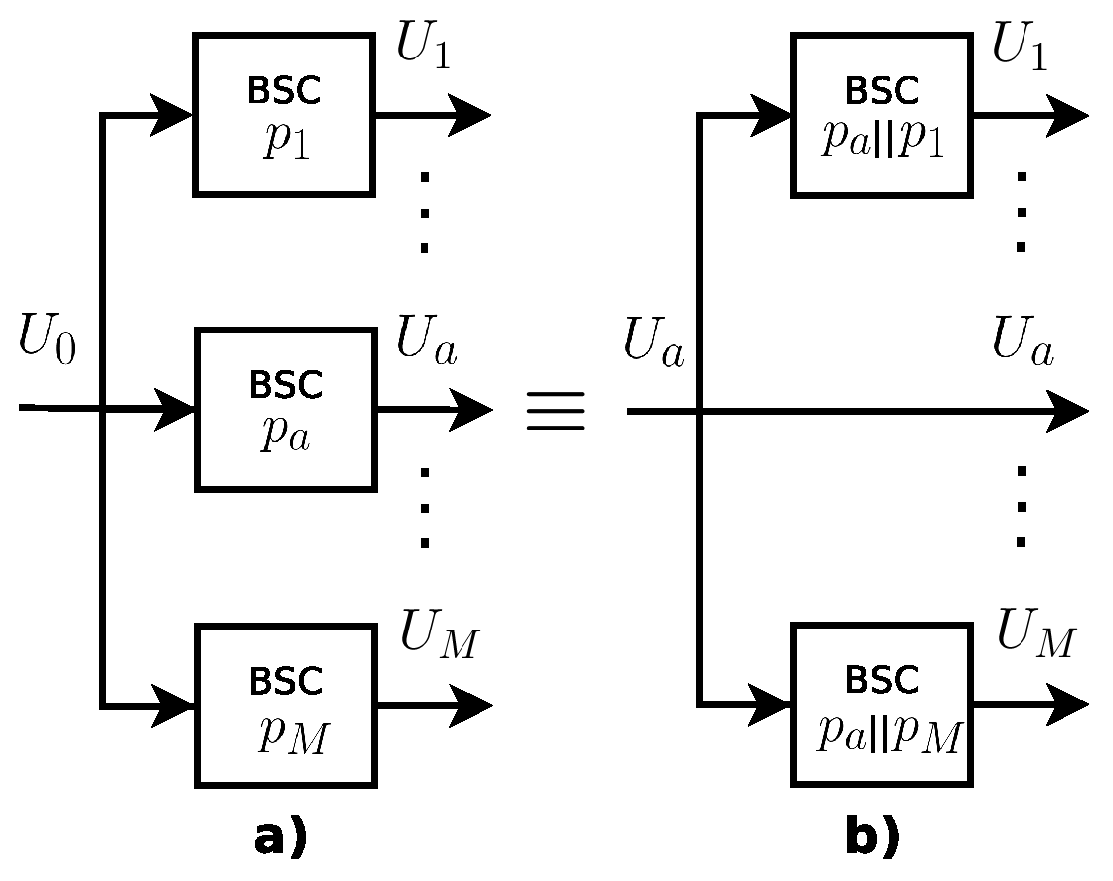
\includegraphics[width=8.0cm]{sources.eps}
\caption{Equivalent Model of correlated sources.} \label{fig:sources}
\end{figure} 
\end{lemma}
\begin{proof}
\label{proof:twoparbsc2} 
Using consecutively the Lemma \ref{lemma:twoparbsc} for all sources $U_m$ in 
the Fig. \ref{fig:sources}a the equivalence is proved.
\end{proof}



%%%%%%%%%%%%%%%%%%%%%%%%%%%%%%%%%%%%%%%%%%%%%%%%%%%%%%%%%%%%%%%%%%%%%%%%%%%%%%
\begin{lemma}
\label{lemma:equivbscldgm_}
Considering a transmit channel as in the 
Fig. \ref{fig:equiv_}a, where we have a source $U_a$ that passes through of a BSC 
channel with error probability $p_m$ and the output is codified with a systematic 
LDGM matrix G, with rate $r$ and $Y$ ones per column in the parity matrix $P$. 
This is statistically  identical to have a source $U_a$ that is codified with 
a matrix $G$ and result pass through two BSC channel in parallel, as is drawn 
in the Fig. \ref{fig:equiv_}b. One BSC channel has a error probability $p_m$ and
work over the $K$ first systematic bits of the codified output, the other BSC
channel of error probability $||^Y p_m$ work over the last $N-K$ codified bits.
\begin{figure}[h!bt]
\centering
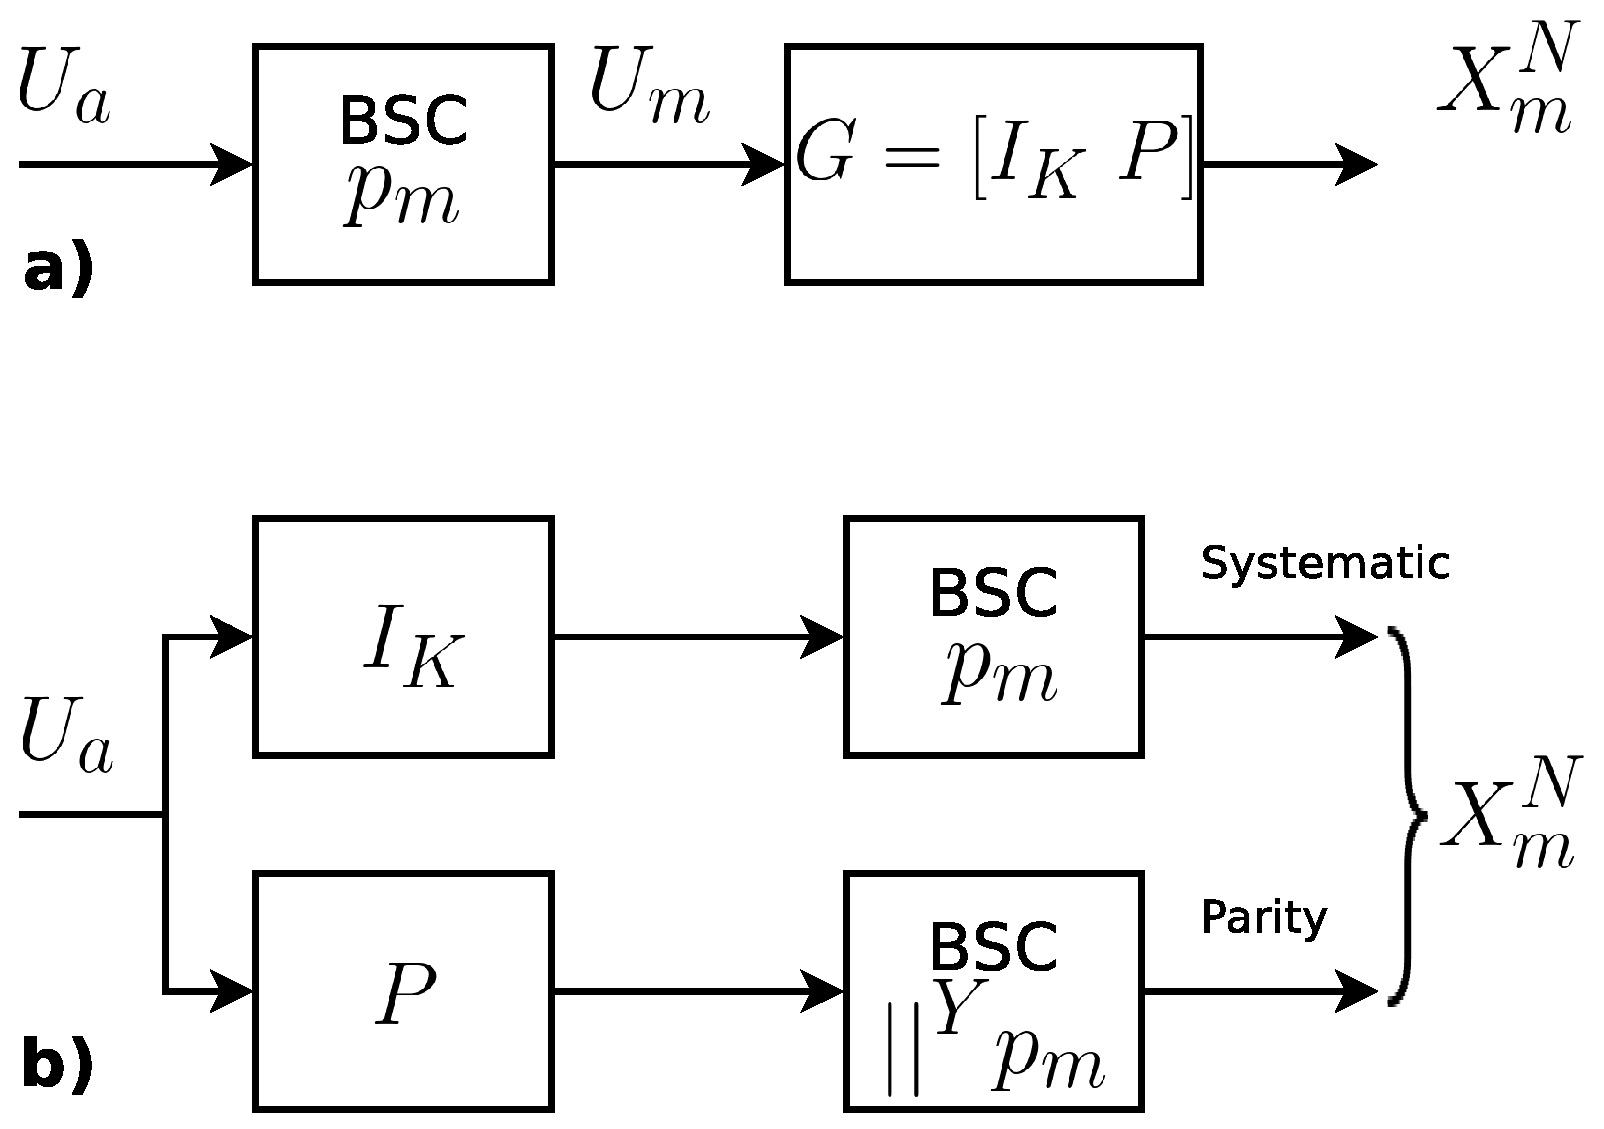
\includegraphics[width=7.5cm]{equiv_.eps}
\caption{Equivalent Model of LDGM Matrix Later of BSC Channel.} \label{fig:equiv_}
\end{figure} 
\end{lemma}
\begin{proof}
\label{proof:equivbscldgm_}
In the Fig \ref{fig:equiv_}a the vector $X^N_m=[$ $x_{m(1)},$ $...,$ $x_{m(K)},$ 
$x_{m(K+1)},$ $...,$ $x_{m(N)}]$ can be seen as a noise codified version of 
vector $U^K_a=[$ $u_{a(1)},$ $...,$  $u_{a(K)}]$ of source $U_a$. The first $K$ 
bits of $X^N_m$ have an error probability $p_m$ and the last $N-K$
bits have an error probability of $\mathring{p}_m$. 
For to calculate $\mathring{p}_m$ first is necessary to define a vector $U^K_m=[$ 
$u_{m(1)},$ $...,$ $u_{m(K)}]$ of source $U_m$ as 
\begin{equation} \label{eq:umemu0_}
u_{m(k)}=u_{a(k)} \oplus e_{m(k)},
\end{equation}
$\forall k \in \{1, 2, ...,K\}$, 
where $e_{m(k)}$ is a element of vector $E^N_{m}=[$ $e_{m(1)},$ $...,$  
$e_{m(K)}]$ with $Pr(E_m=1)=p_m$ and $\oplus$ is the operator XOR.
Thus, each coded bit in $x_{m(n)}$, $\forall n \in \{K+1, K+2, ...,N\}$, is 
equal to
\begin{align}\label{eq:xmn00_}
x_{m(n)} &= \sum^{\oplus}_{l \in \varphi_n } { u_{m(l)} }                \\ 
~        &= \sum^{\oplus}_{l \in \varphi_n } { u_{a(l)} } \oplus \sum^{\oplus}_{l \in \varphi_n } {e_{m(l)}},
\end{align}
where $\sum^{\oplus}$ is a XOR summatory and $\varphi_n$ is a subset with the 
index bits for calculate to $n$-th parity check bit $x_{m(n)}$ using the parity 
matrix $P$. $\varphi_n$ has $Y$ elements. Thus, the error probability 
$\mathring{p}_m$ is equal to 
\begin{equation} \label{eq:dotpm_}
\mathring{p}_m= Pr(\sum^{\oplus}_{l \in \varphi_n } {e_{m(l)}}=1).
\end{equation}
Using the Lemma \ref{lemma:xor} for $Y$ sources independents and identically 
distributed 
\begin{equation} \label{eq:dotpm2_}
\mathring{p}_m= ||^Y p_m.
\end{equation}
Know it can be say that in the Fig. \ref{fig:equiv_}b
the first $K$ bits have an error probability $p_m$ and the last $N-K$ an error 
probability $\mathring{p}_m$.
\end{proof}
%%%%%%%%%%%%%%%%%%%%%%%%%%%%%%%%%%%%%%%%%%%%%%%%%%%%%%%%%%%%%%%%%%%%%%%%%%%%%%%
\begin{lemma}
\label{lemma:equivsystemmodel}
Known $M$ correlated binary sources $U_m$, $\forall m \in \{1, 2, ..., M\}$ that
transmit information over $M$ BSC channels, as in the Fig. \ref{fig:modelo}. If 
we considering a source $U_a$, $a \in \{1, 2, ..., M\}$, as the generator common 
source of all other sources, the system transmission model of Fig. \ref{fig:modelo}
is equivalent to model in Fig. \ref{fig:equivchannel}. Where 
\begin{equation} \label{eq:hpctm}
\hat{p}_{c_{m}}=p_a||p_m||p_{c_m},
\end{equation}
\begin{equation} \label{eq:tpctm}
\tilde{p}_{c_{m}}=(||^Y (p_a||p_m))||p_{c_m},
\end{equation}
for all value of $m \in \{1, 2, ..., M \}$ so that $m \neq a$. In the case of 
$m=a$ 
\begin{equation} \label{eq:hpcta}
\hat{p}_{c_{a}}=p_a,
\end{equation}
\begin{equation} \label{eq:tpcta}
\tilde{p}_{c_{a}}=p_a.
\end{equation}
\begin{figure}[h!bt]
\centering
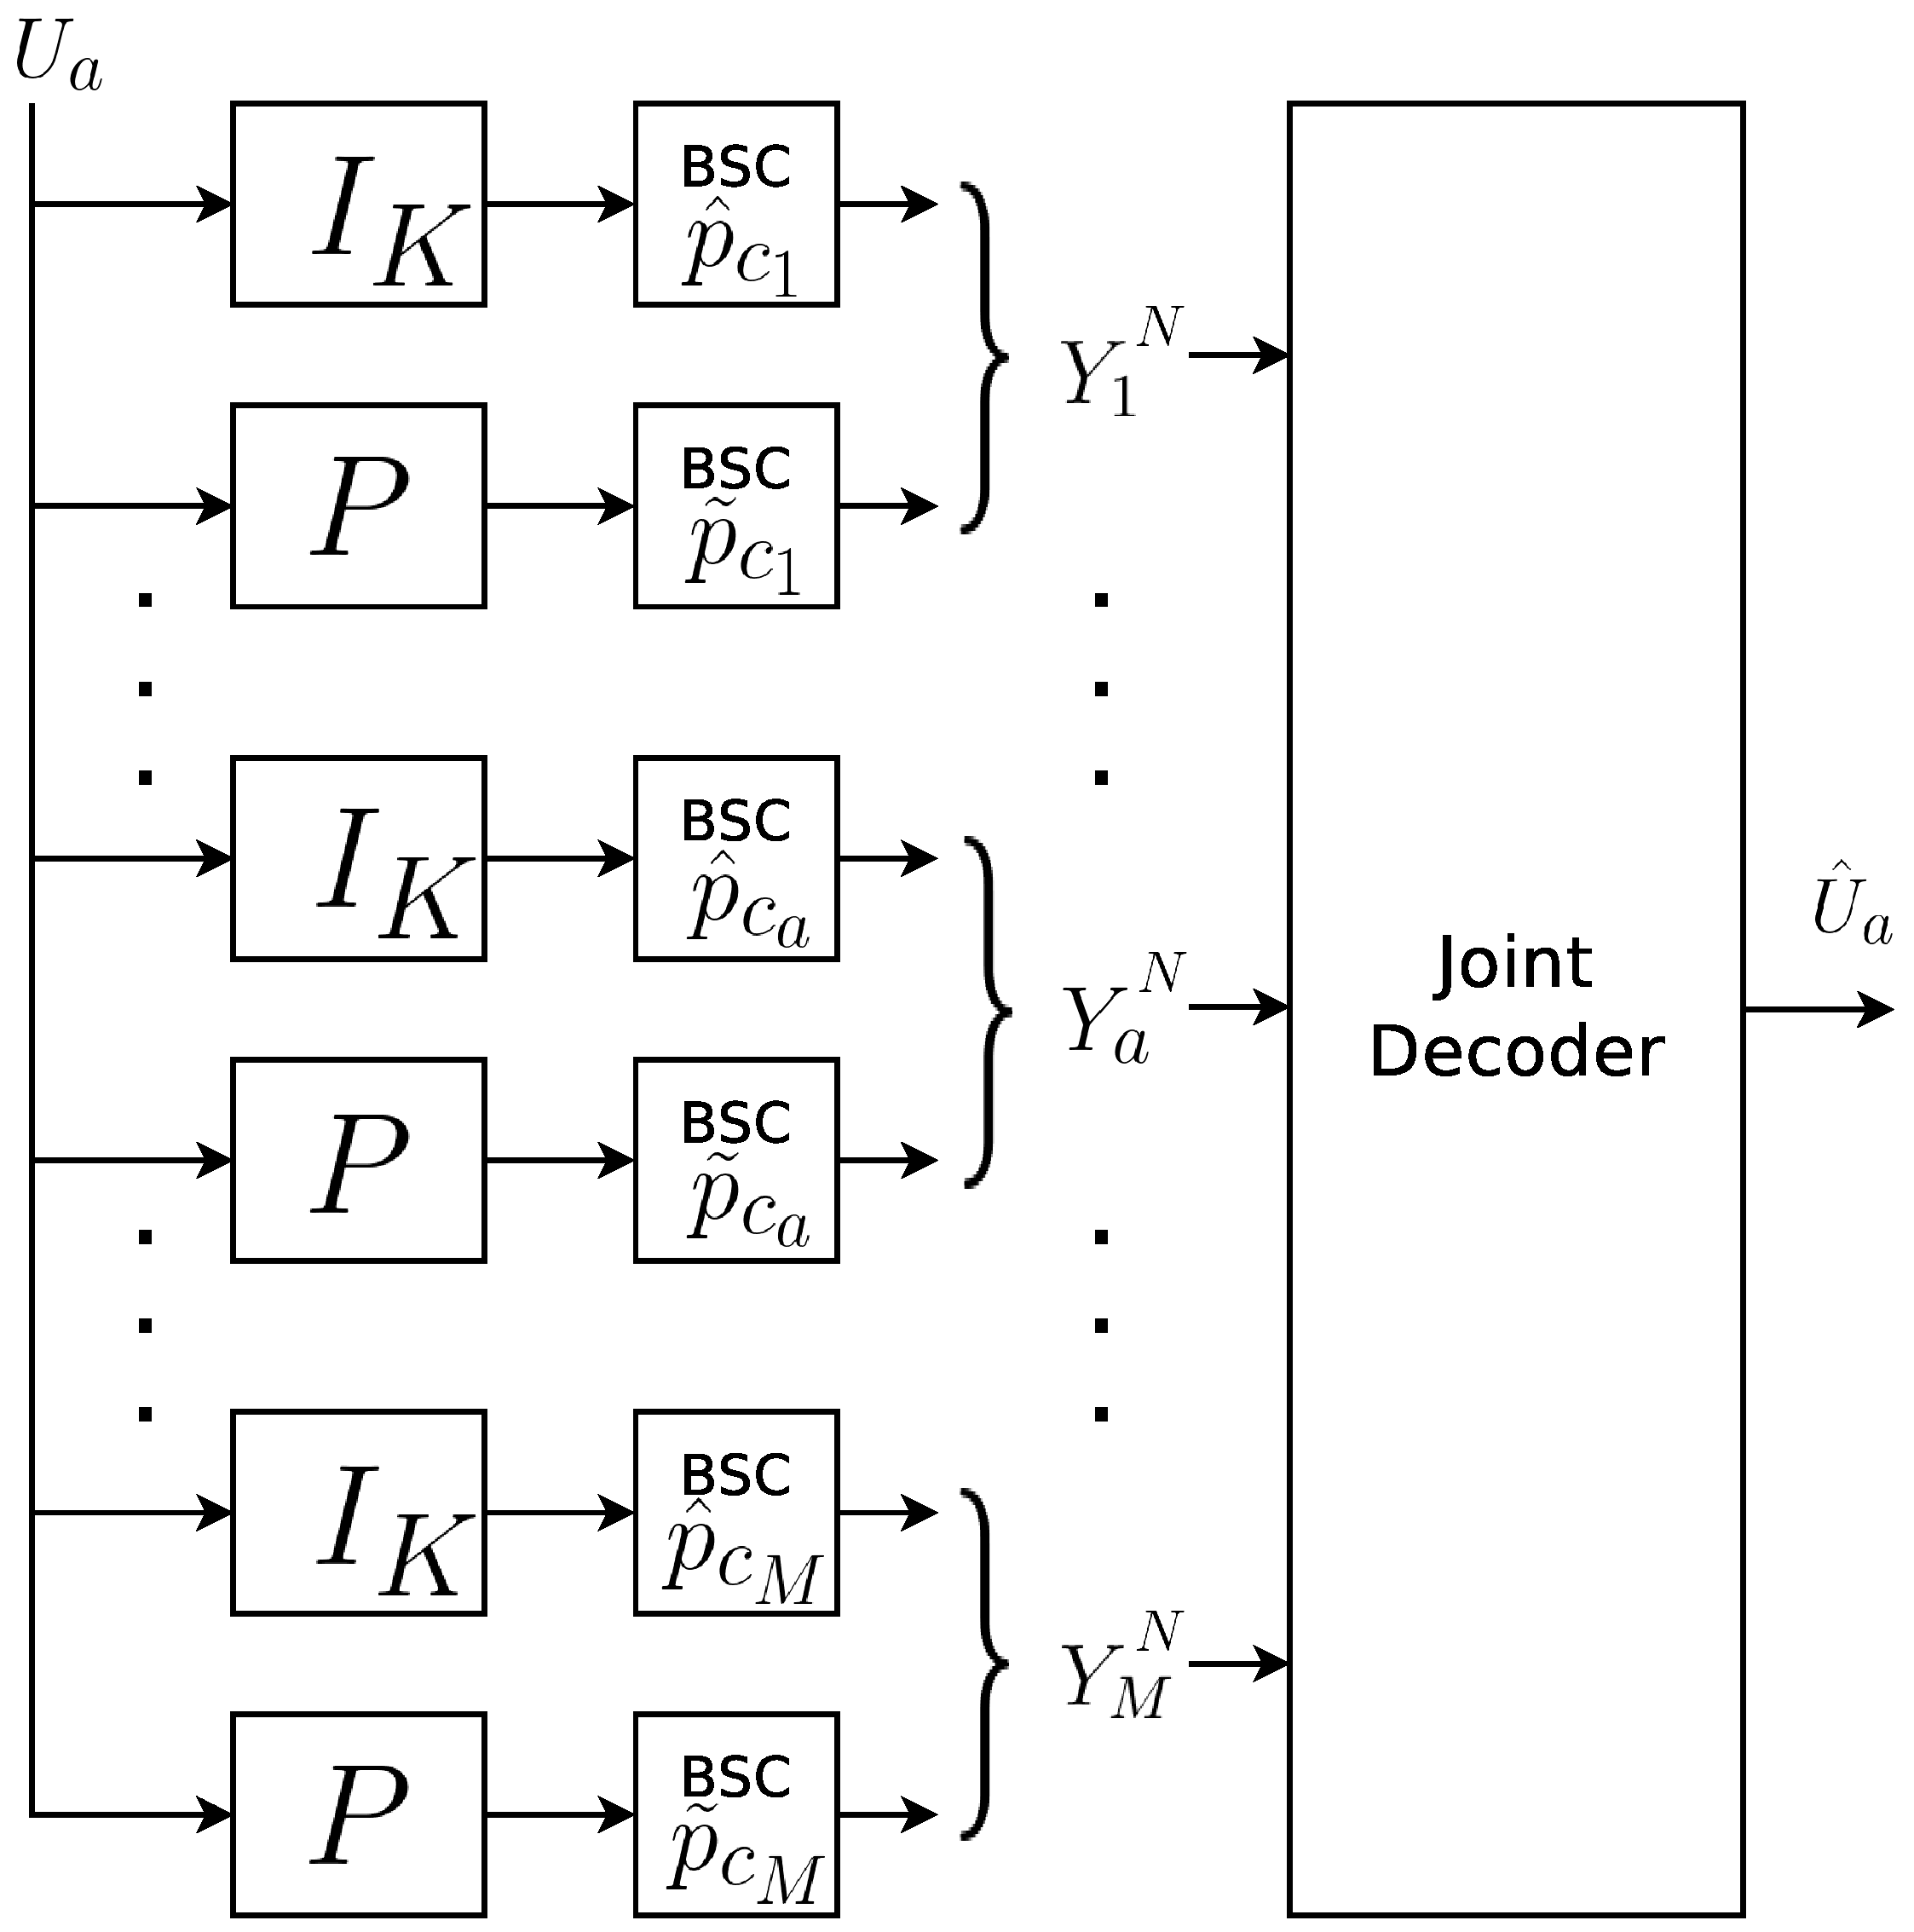
\includegraphics[width=8.0cm]{equiv1.eps}
\caption{Equivalent model of transmission system.} \label{fig:equivchannel}
\end{figure} 
\end{lemma}

%%%%%%%%%%%%%%%%%%%%%%%%%%%%%%%%%%%%%%%%%%%%%%%%%%%%%%%%%%%%%%%%%%%%%%%%%%%%%%
%%%%%%%%%%%%%%%%%%%%%%%%%%%%%%%%%%%%%%%%%%%%%%%%%%%%%%%%%%%%%%%%%%%%%%%%%%%%%%
%%%%%%%%%%%%%%%%%%%%%%%%%%%%%%%%%%%%%%%%%%%%%%%%%%%%%%%%%%%%%%%%%%%%%%%%%%%%%%
\section{Performance  Limit of Systematic LDGM Codes} 
\label{sec:Performance}
~\\
In \cite{art-garciafrias} can be seen a lower bound limit in the prediction 
of the BER for the sources $U_a$, $\forall a \in \{1, 2, ..., M\}$, 
in the case of systematic LDGM codes over BSC channels.
This BER is giving for $Pr(U_a \neq \hat{U}_a)$ and it is in function of the 
quantity of ones for line $X$ in the parity matrix  $P$ and the channel error 
probability $p_c$, where
 \small
 \begin{multline}\label{eq:gf1}
f(X,p_c) \approx \\ \left \{ \begin{matrix}
\sum\limits_{i=\frac{X+1}{2}}^{X} { \binom{X}{i} p_c^i (1-p_c)^{X-i} }  & \text{ if } X~odd \\ 
~ & ~\\
\binom{X}{\frac{X}{2}} p_c^{\frac{X}{2}} (1-p_c)^{\frac{X}{2}} + \sum\limits^{X}_{i=\frac{X}{2}+1} { \binom{X}{i} p_c^i (1-p_c)^{X-i} } & \text{ if } X~even 
\end{matrix} \right .
\end{multline},
\normalsize
\begin{equation}\label{eq:gf3}
 Pr(U_a \neq \hat{U}_a) = f(X,p_c).
\end{equation}
xxxxxxxxxxxxxxxxxxxxxxxxxxxxxxxxxxxxxxxxxxxx\\
Known that
\begin{equation}\label{eq:alg1}
 D_a=\left \{ 
 \begin{matrix}
P_{LLR_a}&= \{& Pr(a_{0})&, ..., Pr(a_{L-1}) &\}  \\
LLR_a  &= \{& a_0    &, ..., a_{L-1}         &\}  
 \end{matrix}
 \right \}
\end{equation}
\begin{equation}\label{eq:alg2}
 g_2(\rho, \gamma)=\left \{ 
 \begin{matrix}
P_{LLR}&= \{& 1-\rho   & \rho    & \}  \\
LLR    &= \{& -\gamma  & +\gamma & \} 
 \end{matrix}
 \right \}
\end{equation}
\begin{equation}\label{eq:alg3}
 sprob(D_a, D_b)=\left \{ 
 \begin{matrix}
P_{LLR}&= P_{LLR_a} \boxdot  P_{LLR_b}   \\
LLR    &= LLR_a     \boxplus LLR_b     
 \end{matrix}
 \right \}
\end{equation}
\begin{equation}\label{eq:alg4}
 prsum(D_a)=\left \{  \sum_{a_i>0} Pr(a_i)\right \}
\end{equation}
\begin{algorithm}
\label{Alg:o1}
 \KwData{$p_c$, $\lambda_{p_c}$, $X$}
 \KwResult{$P_{BER}$:The probability of that the sum of all LLR being major that zero. }
 \BlankLine
 \emph{$D_x=g_2(p_c, \lambda_{p_c})$, $\forall x$ $\in \{1, 2, ..., X\}$}\;
 \emph{$a=2$}\;
 \emph{$D=D_1$}\; 
 \While{$a$ $\leq$ $X$}{
  $D=sprob(D, D_a)$\;
 }
 \emph{$P_{BER}=prsum(D)$}\; 
 \caption{Equivalent algorithm for equation (\ref{eq:gf1})}
\end{algorithm}

In the Algorithm \ref{Alg:o1} the data $D$, in the last result, has $2^X$ elements.
\subsection{Joint Performance Limit of Systematic LDGM Codes}

 \begin{equation}\label{eq:hG}
 \begin{matrix}
\hat{G} & = & [I_K & \hat{P} & ]\\
~       & = & [I_K & \overbrace{P ~ \dots ~ I_K ~ P ~ \dots  ~ I_K ~ P} & ]
\end{matrix}
\end{equation}
 \begin{equation}\label{eq:hH}
\hat{H}^T=\left[ \begin{matrix}
P       & \dots  & I_K    & P       & \dots  & I_K    & P       \\
I_{N-K} & \dots  & 0      & 0       & \dots  & 0      & 0       \\
\vdots  & \ddots & \vdots & \vdots  & \ddots & \vdots & 0       \\
0       & \dots  & I_K    & 0       & \dots  & 0      & 0       \\
0       & \dots  & 0      & I_{N-K} & \dots  & 0      & 0       \\
\vdots  & \ddots & \vdots & \vdots  & \ddots & \vdots & 0       \\
0       & \dots  & 0      & 0       & \dots  & I_K    & 0       \\
0       & \dots  & 0      & 0       & \dots  & 0      & I_{N-K} \\
\end{matrix} \right]
\end{equation}

%%%%%%%%%%%%%%%%%%%%%%%%%%%%%%%%%%%%%%%%%%%%%%%%%%%%%%%%%%%%%%%%%%%%%%%%%%%%%%
%%%%%%%%%%%%%%%%%%%%%%%%%%%%%%%%%%%%%%%%%%%%%%%%%%%%%%%%%%%%%%%%%%%%%%%%%%%%%%
%%%%%%%%%%%%%%%%%%%%%%%%%%%%%%%%%%%%%%%%%%%%%%%%%%%%%%%%%%%%%%%%%%%%%%%%%%%%%%
\section{Final Remarks and Conclusions} 
\label{sec:Conclusions}
The

%%%%%%%%%%%%%%%%%%%%%%%%%%%%%%%%%%%%%%%%%%%%%%%%%%%%%%%%%%%%%%%%%%%%%%%%%%%%%%
%%%%%%%%%%%%%%%%%%%%%%%%%%%%%%%%%%%%%%%%%%%%%%%%%%%%%%%%%%%%%%%%%%%%%%%%%%%%%%
%%%%%%%%%%%%%%%%%%%%%%%%%%%%%%%%%%%%%%%%%%%%%%%%%%%%%%%%%%%%%%%%%%%%%%%%%%%%%%
%\section*{Acknowledgment}
%This work was supported in part by The State of Sao Paulo Research Foundation (FAPESP) under grant 2012/22641-5.

%%%%%%%%%%%%%%%%%%%%%%%%%%%%%%%%%%%%%%%%%%%%%%%%%%%%%%%%%%%%%%%%%%%%%%%%%%%%%%
%%%%%%%%%%%%%%%%%%%%%%%%%%%%%%%%%%%%%%%%%%%%%%%%%%%%%%%%%%%%%%%%%%%%%%%%%%%%%%
%%%%%%%%%%%%%%%%%%%%%%%%%%%%%%%%%%%%%%%%%%%%%%%%%%%%%%%%%%%%%%%%%%%%%%%%%%%%%%
\begin{thebibliography}{99}


\bibitem{ceobinary1} Haghighat, J.; Behroozi, Hamid; Plant, D.V., 
``Iterative joint decoding for sensor networks with binary CEO model,'' 
Signal Processing Advances in Wireless Communications, 2008. SPAWC 2008. 
IEEE 9th Workshop on , vol., no., pp.41,45, 6-9 July 2008.

\bibitem{ceobinary2} Ferrari, G.; Martalo, M.; Abrardo, A.; Raheli, R., 
``Orthogonal multiple access and information fusion: How many observations are needed?,'' 
Information Theory and Applications Workshop (ITA), 2012 , vol., no., pp.311,320, 5-10 Feb. 2012.


\bibitem{cover}
T. M. Cover, and J. Thomas, \textit{Elements of Information Theory}, Wiley-Interscience, 2006.


\bibitem{art-garciafrias} J. F. Garcia-Frias e W. Zhong, \emph{Approaching Shannon performance by
iterative decoding of linear codes with low-density generator matrix,}
~\textit{IEEE Commun. Lett.}, v. 7, n. 6, pp. 266-268, Junho 2003.


\end{thebibliography}

\end{document}


